\documentclass[conference]{IEEEtran}
\IEEEoverridecommandlockouts
% The preceding line is only needed to identify funding in the first footnote. If that is unneeded, please comment it out.
\usepackage{cite}
\usepackage{amsmath,amssymb,amsfonts}
\usepackage{algorithmic}
\usepackage{graphicx}
\usepackage{textcomp}
\usepackage{xcolor}
\usepackage{mathtools}
\usepackage{tabu}
\usepackage{subcaption}
\DeclareMathOperator*{\argmax}{argmax} % thin space, limits underneath in displays
\def\BibTeX{{\rm B\kern-.05em{\sc i\kern-.025em b}\kern-.08em
    T\kern-.1667em\lower.7ex\hbox{E}\kern-.125emX}}
\begin{document}
\title{Variational Inference of Finite Generalized Gaussian Mixture Models\\
}
\author{\IEEEauthorblockN{1\textsuperscript{st} Srikanth Amudala}
\IEEEauthorblockA{\textit{Concordia Institute for Information Systems Engineering} \\
\textit{Concordia University}\\
Montreal, Canada \\
srikanth.amudala@mail.concordia.ca}
\and
\IEEEauthorblockN{2\textsuperscript{nd} Samr Ali}
\IEEEauthorblockA{\textit{Department of Electrical and Computer Engineering} \\
\textit{Concordia University}\\
Montreal, Canada \\
al\_samr@encs.concordia.ca}
\and
\IEEEauthorblockN{3\textsuperscript{rd} Fatma Najar}
\IEEEauthorblockA{\textit{Concordia Institute for Information Systems Engineering} \\
\textit{Concordia University}\\
Montreal, Canada \\
f\_najar@encs.concordia.ca}
\and
\IEEEauthorblockN{4\textsuperscript{th} Nizar Bouguila}
\IEEEauthorblockA{\textit{Concordia Institute for Information Systems Engineering} \\
\textit{Concordia University}\\
Montreal, Canada \\
nizar.bouguila@concordia.ca}
}
\maketitle

\begin{abstract}
    This paper presents a variational inference method to analyze finite generalized Gaussian mixture models (GGMM) which incorporate several standard mixtures widely used in signal and image processing applications, such as Laplace and Gaussian. Our work is motivated by the fact that the generalized Gaussian distribution (GGD) can be applied on different types of data due to its shape flexibility. We present a method to evaluate the posterior distribution and Bayes estimators using variational expectation-maximization algorithm. 
    % The algorithm is based on treating the shape parameter as a variable. Subsequently using Binomial Expansion with two cases, we estimate the expectation of the distributions with power parameter.
    % On this basis, the variational E-step and the variational M-step are performed alternatively to infer the posteriors of the variables and estimate the parameters. 
    The effective number of components of the GGMM is determined automatically. The experimental results demonstrate the effectiveness of the proposed algorithm by applying it to
    medical, astrological, and image segmentation applications; while comparing it to different other approaches.    
\end{abstract}

% \begin{IEEEkeywords}
% component, formatting, style, styling, insert
% \end{IEEEkeywords}

\section{Introduction}
Statistical inference plays a vital role in many research areas such as computer vision, signal processing, and pattern recognition. In particular, mixture models have been widely deployed. Challenges in fitting finite mixture models include identifying the appropriate probability density function as well as the corresponding optimal number of components. 
Gaussian distribution has been widely used and studied with success for many applications involving computer vision, machine learning, image processing and statistical analysis.
% which has to happen the most used and well-fitted distribution with the limitation of the symmetric shape of the Gaussian component density. However, many statistical applications like signal processing or image segmentation where there a tailed peek or asymmetric shape which would require many components for a GMM to account for such a distribution is not feasible.
However, in many real applications, Gaussian distribution fails to fit different shapes of data\cite{b5}.

Recently alternative techniques have been reported in the literature to resolve the Gaussian assumption limitation. 
The generalized Gaussian distribution (GGD) has been proposed
to provide more flexibility, by introducing a new parameter called shape parameter.  
The GGD has three special cases with respect to the varying shape parameter namely the Laplacian, the Gaussian, and the asymptotically uniform distributions. 

For instance, generalized Gaussian mixture model (GGMM) has been used in \cite{n15} for buffer control, in \cite{n16, n17, n18} for texture classification and retrieval, in \cite{n27, n28, n29} for video and image segmentation, in \cite{n13} for multiresolution transmission of high-definition video, in \cite{n30} for SAR images statistics modelling, in \cite{n14} for subband decomposition of video,   in \cite{n19} for denoising applications, in \cite{n20, n21} for data and image compression, in \cite{n22} for edge modeling, in \cite{n23, n24} for image thresholding, in \cite{n12, n4} to fit subband histograms, in \cite{n25, n26} for speech modeling,  and in \cite{n31} for multichannel audioresynthesis.
Several methods have been proposed to estimate the parameters of GGMM such as entropy matching estimation \cite{n34, n26} and maximum likelihood estimation \cite{n32, n16, n35, n36, n10} with a deterministic approach where a single distribution is considered. 
Maximum likelihood estimation is performed via the Expectation Maximization (EM) algorithm which has gained attention in recent times with its lower computational time. However, the EM algorithm is known for its convergence to local maxima and the tendency to overfit the model.

An alternative technique that has been gaining attention in the literature is the Bayesian method, for which a Markov chain Monte Carlo (MCMC) technique has been proposed in \cite{nb1}. Although the MCMC algorithm yields better results for the inference of the GGMM, it is computationally intensive to evaluate the simulation-based estimator due to the Gibbs and Metropolis Hastings sampling.

In order to tackle problems related to both Bayesian and deterministic estimation, we propose in this paper a variational approach. 
% a Bayesian inference approach for the GGMM within the framework of Variational Expectation Maximization (VEM) \cite{g1}. 
By considering possible distributions we assign appropriate priors to the mean and the precision of GGMM. We do not assign any prior distribution to the shape parameter of the GGMM to appropriately derive closed-form expressions. 
With the well defined prior distributions, the lower bound of the variational objective function is constructed. This facilitates the derivation of the closed-form updates in the variational expectation step (VE-step).
Adopting the single-step update of Newton's method from \cite{g2}, the closed-form updates for the power parameters are achieved in the variational maximization step (VM-step).
By performing alternatively the VE-step and the VM-step, all the parameters of the GGMM are updated.
Experiments are performed based on medical, astrological, and image data sets to verify the effectiveness of the proposed method.

This paper is organized as follows. In Section 2, we present the variational inference of GGMM. 
In Section 3, we
evaluate the performance of the proposed model on classification and segmentation applications.
We conclude the paper in Section 4.

\section{Variational Inference of the Generalized Gaussian Mixture Model}

\subsection{Generalized Gaussian Mixture Model}
The one-dimensional GGMM for a variable $\mathcal{X} \epsilon R $ with parameters $\mu, \tau, \lambda$ is defined as follows:
\begin{equation}
    \begin{split}
        P(\mathcal{X}|\mu, \tau, \lambda) &= \frac{\lambda  \tau^\frac{1}{\lambda}}{2\Gamma(\frac{1}{\lambda})}
          e^{-\tau  |(\mathcal{X}-\mu)|^{\lambda}}    
        %   \text{where, }
        % \tau &= \Bigg({\frac{1}{\sigma} \sqrt{\frac{\Gamma(\frac{3}{\lambda})}{\Gamma(\frac{1}{\lambda})}}}\Bigg)^\lambda
    \end{split}
    \end{equation}
where $\tau = \bigg({\frac{1}{\sigma} \sqrt{\frac{\Gamma(\frac{3}{\lambda})}{\Gamma(\frac{1}{\lambda})}}}\bigg)^\lambda$, $\Gamma(.)$ denotes the gamma function given by $\Gamma(z) = \int_{0}^{\infty}p^{z-1}e^{-p} dp$, where $z$ and $p$ are real variables.
The parameters $\mu, \sigma, \lambda$  denote the mean, standard deviation and the shape parameter, respectively. The parameter $\lambda$ controls the shape of the probability density function.
The larger the value, the flatter the probability density function. This means that $\lambda$ determines the decay rate of the density function. 
Note that for the two special cases, when $\lambda = 2$ and $\lambda = 1$, the GGD is reduced to the Gaussian and the Laplacian distributions, respectively.
If $\mathcal{X}$ follows a mixture of $K$ GGDs, then 
\begin{equation}
    P(\mathcal{X}|\Theta) = \sum_{k = 1}^{K} P(\mathcal{X}|\mu_k, \tau_k, \lambda_k)\pi_k
\end{equation}


where $\pi_k(0\leq\pi_k\leq1$ and $\sum_{k=1}^{K} \pi_k = 1)$ are the mixing weights and $p(\mathcal{X}|\mu_k, \tau_k, \lambda_k)$ is the GGMM likelihood of component $k$. 
As for the symbol $\Theta = (\epsilon, \pi)$, it refers to the entire set of parameters to be estimated where $\epsilon = (\mu_1, \tau_1, \lambda_1, ..., \mu_K, \tau_K, \lambda_K)$ and $\pi=(\pi_1,...,\pi_K)$. 

Considering $N$ observations,  $\mathcal{X} = (X_1, X_2, ..., X_N)$, and supposing that the number of components $K$ is known, the data likelihood is denoted as follows:
\begin{equation}
    P(\mathcal{X}|\Theta) = \prod_{n = 1}^{N}\sum_{k=1}^{K} P({X}_n|\epsilon_k)\pi_k
\end{equation}
where $\epsilon_k = (\mu_k, \tau_k, \lambda_k)$. 
For each variable ${X}_i$, let $Z_i$  be $K$-dimensional vector known by the unobserved vector that assigns the appropriate mixture component ${X}_i$ belongs to. Then, $Z_{ik}$ is equal to 1 if ${X}_i$ belongs to class $k$ and 0, otherwise. Hence, the complete-data likelihood is given by:
\begin{equation}
    P(\mathcal{X}|\Theta) = \prod_{n = 1}^{N}\sum_{k=1}^{K} (P({X}_n|\epsilon_k)\pi_k)^{Z_{nk}}
\end{equation}
% where $Z =(Z_1, Z_2, ..., Z_N)$

The EM algorithm comprises of finding the mixture parameters that maximize the complete data log-likelihood given by:
\begin{equation}
    L(\mathcal{X}, Z, \Theta) = \sum_{n = 1}^{N}\sum_{k=1}^{K} Z_{nk}\ln(P(X_n|\epsilon_k)\pi_k)
\end{equation}
The assignment of $k^{th}$ component of the mixture can be denoted as follows\cite{b9}:
\begin{equation}
    \hat{Z}_{nk}^t = \frac{P^{t-1}(X_n|\epsilon_k^{t-1})p_k^{t-1}}{\sum_{k=1}^{K} P^{t-1}(X_n|\epsilon_k^{t-1}) p_k^{t-1}}
\end{equation}
where $t$ denotes the current step and $\epsilon_k^t$ and $p_j^t$ are the current estimates of the parameters.
The EM algorithm produces a sequence of estimates to the mixture parameters $\Theta^t$, for $t=0,1,...,$ until a convergence measure is fulfilled through two distinctive steps: the expectation and the maximization. The EM algorithm comprises of:
\begin{enumerate}
    \item Initialization of the mixture parameters.
    \item E-step: Compute $\hat{Z}^t_{nk}$ (Eq. (6)) using the initialized
    parameters.
    \item M-step: Update the parameters using \\
        $\hat{\Theta}^t =$ $\argmax_{z_{\Theta}}$ $L(\Theta, Z, \mathcal{X})$.
\end{enumerate}

We note that the EM algorithm has some drawbacks, like convergence to local maxima due to its dependence on initialization. 
A detailed discussion of the disadvantages of the EM algorithm is in \cite{b1}.
% An extension to the EM algorithm based on the execution of the E-step by Monte Carlo, 
% called Markov chain Monte Carlo (MCEM), has been proposed in \cite{b2}. 
% Although the Markov chain Monte Carlo (MCMC) algorithm yields better results for the inference of the GGMM, it is computationally intensive to evaluate the simulation-based estimator due to the Gibbs and Metropolis sampling. 
% Moreover, both the MCMC-based method and the EM-based methods fail to address the model complexity problem (i.e., the selection of the number of components) in the GGMM.

% To achieve both the closed-form updates and the automatic determination of component number, we propose a Bayesian inference approach for the Generalized Gaussian Mixture Model within the framework of variational expectation maximization (VEM) \cite{b10}\cite{b11}.
% An efficient alternative technique that we will propose in the following is the Variational approach which has received a lot of attention in recent times.
\subsection{Variational Inference of the Generalized Gaussian Mixture Model}

We propose a variational inference approach for the GGMM within the framework of Variational Expectation-Maximization (VEM) \cite{b10} \cite{Bishop} to achieve the closed-form updates and automatic determination of the number of mixture components by 
optimizing the Kullback–Leibler (KL) divergence between the true posterior $p$ and the approximate distribution $q$ \cite{Bishop}.
The smaller the KL divergence, the stronger the relationship between the distributions. The KL divergence is denoted by:
\begin{equation}
    \begin{split}\label{kl}
    KL(p\parallel q) & = - \int q(Z) \ln\{\frac{p(Z,\mathcal{X})}{q(Z)}-\ln p(\mathcal{X})\}dZ \\ &
    = - \int q(Z) \ln\{\frac{p(Z,\mathcal{X})}{q(Z)}\}dZ + \ln p(\mathcal{X})
    \end{split}
 \end{equation}
 In order to calculate the KL divergence, we need to calculate the evidence $\ln p(\mathcal{X})$. This is difficult to calculate which motivates the proposed variational inference approach.
 Reordering Eq. (\ref{kl}), we get: 
 \begin{equation}
    \ln p(\mathcal{X}) = KL(p\parallel q) + \underbrace{\int q(Z) \ln\{\frac{p(Z,\mathcal{X})}{q(Z)}\}dZ}_\text{Evidence Lower Bound}
 \end{equation}
Maximizing the Evidence Lower Bound (ELBO) is equivalent to minimizing the KL divergence. 
By applying Jensen's inequality, the ELBO serves as a lower-bound for the log-evidence, $\ln p(\mathcal{X}) \geq$ ELBO$(q)$ for any $q(Z)$, which is
the approximate of the posterior.  
In order to maximize the ELBO, we need to choose a variational family $q$.
The complexity of the family determines the flexibility in providing appropriate approximation to the true posterior distribution.



We assign Normal priors for the distributions mean, and Gamma
priors for the precision and shape parameters [47,48]:
$\mu_k \sim N(\mu| m_0, s_0^{-1}), \tau_k \sim G(\tau|\alpha_0, \beta_0), \lambda_k \sim G(\lambda|\alpha_{\lambda}, \beta_{\lambda})$ where $N(\mu| m_0, s_0^{-1})$
is the Normal distribution with mean $m_0$ and precision $s_0^{-1}$, $G(\tau|\alpha_0, \beta_0)$
is the Gamma distribution with shape parameter
$\alpha_0$ and rate parameter $\beta_0$, $\lambda$, $\mu_0, s_0, \beta_0, \alpha_0$ are the 
hyperparameters of the model.
With these priors, the posterior distributions for $\mu, \tau, \lambda$ are defined as \cite{b9}:
\begin{equation}
    \begin{split}
        p(\mu_k|Z, X) &\propto e ^{{-(\mu_k - \mu_0)^2 s_0/2} + \sum_{Z_{nk} = 1} - (\tau_k|X_n - \mu_k|)^{\lambda_k}}   \\
        p(\tau_k|Z, X) &\propto \alpha_k ^{\alpha_0 - 1} e ^{-\beta_0 \tau_k}\tau_k^{n_j} e ^{\sum_{Z_{nk} = 1} - (\tau_k|X_n - \mu_k|)^{\lambda_k}}   \\
        p(\lambda_k|Z, X) &\propto \lambda_k ^{\alpha_\lambda - 1} e ^{-\beta_\lambda \lambda_k}\tau_k^{n_j}\bigg(\frac{\lambda_k}{\Gamma(1/\lambda_k)}\bigg)^{n_j} \\
        &e ^{\sum_{Z_{nk} = 1} - (\tau_k|X_n - \mu_k|)^{\lambda_k}}  
    \end{split}
\end{equation}
Accordingly, we can not use the posterior distributions in their current state. 
% \subsection{Proposed VE interface of GGMM}

% PDF of Generalised Gaussian Mixture model
% \begin{equation}
%     \begin{split}
%         P(X|\mu_k, \tau_k, \lambda_k) &= \frac{\lambda_k  \tau_k^\frac{1}{\lambda_k}}{2\Gamma(\frac{1}{\lambda_k})}
%           exp(-\tau_k  |(X-\mu_k)|^{\lambda_k})    \\
%         \tau &= (\frac{1}{\sigma} \sqrt(\Gamma(\frac{3}{\lambda})/\Gamma(\frac{1}{\lambda})))^\lambda
%     \end{split}
%     \end{equation}
    
    % \begin{equation}
    % \tau = (\frac{1}{\sigma} * \sqrt(\Gamma(\frac{3}{\lambda})/\Gamma(\frac{1}{\lambda})))^\lambda
    % \end{equation}

    % In order to formulate  the variational inference model, we denote
% the joint distribution of all of the random variables assuming all parameters are independent as can be observed in Fig. 1. 
To formulate the variational inference model, we denote
the joint distribution of all the random variables assuming all parameters are independent as can be observed in Fig. 1: 
\begin{equation}
    p(X, Z, \pi, \mu, \tau, \lambda) = p(X|Z, \mu, \tau, \lambda)p(Z|\pi)p(\pi)p(\mu)p(\tau)p(\lambda)
\end{equation}
\begin{figure}[h!]
    \begin{center}
        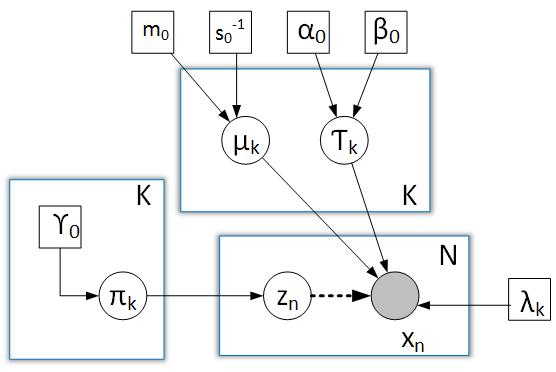
\includegraphics[width=0.7\linewidth]{imgresults/model.jpeg}
        \caption{Graphical model for the VGGM. 
        The filled circle, unfilled circles and squares represent observations, random variables, and parameters, respectively. The dependency among the variables is represented by directional arrows.}
        \label{VGGM Graphical Model}    
    \end{center}
\end{figure}

Because of the nonlinearity of the shape parameter, the conjugate prior distribution can not be directly found. Therefore, we considered using the Taylor approximation to find an 
approximate lower bound of the complete-data log-likelihood to determine whether an appropriate prior exists in the exponential family. 
However, the negative second order derivative causes the function $q(\lambda)$ to be concave, resulting in an upper bound rather than a lower bound; which is required.
Hence, we consider $\lambda$ as a parameter and it is not assigned a prior distribution\cite{b5}. 
The conjugate exponential priors for $\mu$ and $\tau$ are Normal and Gamma distributions. Therefore, we specify all the priors according to:
\begin{equation}
    \mu_k \sim N(\mu| m_k, s_k^{-1})   
\end{equation}
\begin{equation}
    \tau_k \sim G(\tau|\alpha_k, \beta_k)    
\end{equation}
We consider a variational distribution which factorizes into the latent
variables and the parameters:
\begin{equation}
    q(Z, \pi, \mu, \tau, \lambda) = q(Z)q(\pi, \mu, \tau, \lambda)
\end{equation}
\begin{equation}
    \ln q^\star(Z) = \mathop{\mathbb{E}_{\mu, \tau, \pi}}[\ln p(\mathcal{X}, \pi,\mu, \tau, \lambda)] + const.
\end{equation}
\begin{equation}
    \begin{split}
        \ln q^\star(Z) = \mathop{\mathbb{E_\pi}}[\ln p(Z|\pi)]+\mathop{\mathbb{E_{\mu, \tau}}}[\ln p(\mathcal{X}|Z,\mu, \tau, \lambda)] + const.
    \end{split}
\end{equation}
where $\mathbb{E}$ represents the expectation with respect to the subscripted parameter and $const$ denotes an additive constant.
Substituting the two conditional distributions, and absorbing any terms that are independent of $Z$ into the additive constant, we have:
\begin{equation}
    \ln q^\star(Z) =  \sum_{\mathclap{n=1}}^{N} \sum_{\mathclap{k=1}}^{K}z_{nk} \ln \rho_{nk} + const
\end{equation}
where we define:
\begin{equation}
    \begin{split}\label{rownk}
        \ln \rho_{nk} = &\mathop{\mathbb{E}_{\pi}}[\ln \pi_k] + \mathop{\mathbb{E}_{\mu, \tau}}[\frac{1}{\lambda_k} \ln \tau_k + \ln \lambda_k - \ln 2\Gamma(1/\lambda_k)\\
        & - \tau_k |X_n - \mu_k|^{\lambda_k}]    
    \end{split}
\end{equation}

Normalizing the distribution, noting for each value of $n$ the values of $Z_{nk}$ are binary and add up to 1 overall values of $k$, we obtain:
\begin{equation}
    q^\star(Z) = \prod_{n=1}^{N}\prod_{k=1}^{K} r_{nk}^{z_{nk}}
\end{equation}
where
\begin{equation}\label{rnk}
    r_{nk} = \frac{\rho_{nk}}{\sum_{k=1}^{K}\rho_{nk}}
\end{equation}

The optimal solution for the factor $q(Z)$ then follows the same functional form
as the prior $p(Z|\pi)$. Note that because $\rho_{nk}$ is given by the exponential of a real
quantity, the quantities $\rho_{nk}$ will be non-negative and will sum to one, as required.
For the discrete distribution $q^\star(Z)$:
\begin{equation}
    \mathop{\mathbb{E}}[z_{nk}] = r_{nk}
\end{equation}
where $r_{nk}$ denotes the responsibilities with the sum of all the responsibilities for the respective cluster $k$ given by $N_k$:
\begin{equation}
    N_k = \sum_{\mathclap{n=1}}^{N}r_{nk}
\end{equation}
Similarly, the factor  in the variational posterior distribution $q(\pi, \mu, \tau, \lambda) $ is given by:
\begin{equation}
    \begin{split}
        \ln q^\star (\pi, \mu, \tau, \lambda) = \ln q(\pi) +  \sum_{k=1}^{K} q(\mu_k, \tau_k, \lambda_k)
    \end{split}
\end{equation}
We observe that this expression decomposes into a sum of
terms with only $\pi$ in addition to terms with $\mu$ and $\tau$, which implies
that the variational posterior $q(\pi, \mu, \tau, \lambda)$ factorizes to:\\
\begin{equation}
    q(\pi, \mu, \tau, \lambda) = q(\pi) \prod_{k=1}^{K} q(\mu_k, \tau_k, \lambda_k)
\end{equation}

% We choose a Dirichlet distribution over the mixing coefficients $\pi$
% \begin{equation}
% p(\pi)= Dir(\pi|\gamma_0)=  \frac{\Gamma(\sum_{k=1}^{K} \gamma_{0})}{\prod_{k=1}^{K} \Gamma(\gamma{0})}\prod_{k=1}^{K} \pi_k^{\gamma-1}
% \end{equation}

Identifying the terms that depend on $\pi$, results in:
\begin{equation}
    \ln q^\star(\pi) = (\gamma_0 - 1)\sum_{k=1}^{K}\ln \pi_k + \sum_{k=1}^{K}\sum_{n=1}^{N} r_{nk} \ln \pi_k + const
\end{equation}
We then recognize $q^\star(\pi)$ as a Dirichlet distribution with parameter $\gamma$:
\begin{equation}
    q^\star(\pi) =  Dir(\pi|\gamma)
\end{equation}
where $\gamma$ has components $\gamma_k$ that are given by:
\begin{equation}\label{gammak}
    \gamma_k = \gamma_0 + N_k
\end{equation}   
    \begin{equation}
        \begin{split}
            \mathop{\mathbb{E}}[\ln \pi_k] &= \psi(\gamma_k) - \psi(\hat{\gamma})\\
            \hat{\gamma} &= \sum_{k=1}^{K} \gamma_k
        \end{split}
    \end{equation}
    The expectation of $\mu$ with prior means $m_0$ and precision $ s_0^{-1}$ are denoted by:
    \begin{align}
    \begin{split}
    \mathop{\mathbb{E}}[\ln q(\mu_k)] = &\mathop{\mathbb{E}_\tau}\bigg[\sum_{\mathclap{n=1}}^{N}(-Z_{nk}\tau_k|X_n - \mu_k|^{\lambda_k}) - \\
    &\frac{s_0}{2}(\mu_k - m_0)^2\bigg]
    % -\frac{s_0}{2} + \sum_{\mathclap{n=1}}^{N}(r_{nk} \tau_k)\bigg]
    \end{split}
    \end{align}
    where $|X_n - \mu_k|^{\lambda_k}$ is expanded using the Binomial Expansion to the power 2 with the following conditions:\\
    $if(\mu_k > X_n )$
    \begin{equation}
        \begin{split}
            |\mu_k - X_n|^{\lambda_k}=&\mu_k^{\lambda_k} - \lambda_k \mu_k^{\lambda_k - 1} X_n +\\
            &\frac{\lambda_k}{2} (\lambda_k - 1) \mu_k^{\lambda_k - 2} X_n^2
        \end{split}
    \end{equation}
    $if(X_n>\mu_k)$
    \begin{equation}
        \begin{split}
            |X_n-\mu_k|^{\lambda_k} &= |X_n|^{\lambda_k}\bigg(1 - \frac{\mu_k}{X_n}\bigg)^{\lambda_k},\\
            \bigg(1 - \frac{\mu_k}{X_n}\bigg)^{\lambda_k} &= 1 - \lambda_k \frac{\mu_k}{X_n} + \frac{\lambda_k}{2}(\lambda_k-1) \frac{\mu_k^2}{X_n^2}
        \end{split}
    \end{equation}
    Substituting Eq. (29) and Eq. (30) in Eq. (28) and comparing it to the prior distribution, we obtain:
    \begin{equation}
        \begin{split}\label{mk}
            m_k = \frac{\frac{s_0m_0}{2} + p_1}
            {s_k}
        \end{split}
    \end{equation}
    \begin{equation}\label{sk}
        s_k = \frac{s_0}{2} + p_2
    \end{equation}
where $p_1, p_2 $ have two different cases as follows:
\[
    p_1= 
\begin{cases}
    \sum_{{n=1}}^{N}(r_{nk}\bar{\tau}_k\frac{\lambda_k}{4}(\lambda_k-1)\mu_k^{\lambda_k-3} x_n^2 + \\ 
        \sum_{{n=1}}^{N}(r_{nk}\bar{\tau}_k\frac{\lambda_k}{2}\mu_k^{\lambda_k-2}x_n))     ,& \text{if } X_n < m_k\\ \\
        \sum_{n=1}^{N}r_{nk}\bar{\tau}_k\lambda_k\frac{|x_n|^{\lambda_k}}{x_n},              & \text{otherwise}
\end{cases}
\]
\[
        p_2= 
    \begin{cases}
        \sum_{{n=1}}^{N}(r_{nk}\bar{\tau}_k\mu_k^{\lambda_k-2}),& \text{if } X_n < m_k\\ \\
        \sum_{{n=1}}^{N}(r_{nk}\bar{\tau}_k\frac{\lambda_k}{2}(\lambda_k-1)\frac{|x_n^{\lambda_k}|}{x_n^2}),              & \text{otherwise}
    \end{cases}
    \]


Where $\bar{\tau}$ represents $\mathop{\mathbb{E}_\tau}[\tau]$.
Similarly, the solution for $\tau$ is as follows:
    \begin{equation}
        \mathop{\mathbb{E}}[\ln q(\tau_k)] = \mathop{\mathbb{E}_\mu}\bigg[\frac{\lambda_k \tau_k^{\frac{1}{\lambda_k}}}{2\Gamma(\frac{1}{\lambda_k})} e ^ {-\tau_k |X-\mu_k|^{\lambda_k}} + \ln\tau_k^{\alpha_0 - 1} - \beta_0 \tau_k\bigg]
    \end{equation}
    \begin{equation}
        \begin{split}\label{alphak}
            \alpha_k = \sum_{\mathclap{n=1}}^{N} r_{nk} + \alpha_0 - 1
        \end{split}
    \end{equation}
    
    \begin{equation}\label{betak}
        \beta_k = \beta_0 + \sum_{\mathclap{n=1}}^{N} r_{nk} \mathop{\mathbb{E}_\mu}[|X_n - \mu_k|^{\lambda_k}]
    \end{equation}
     \[
        \mathop{\mathbb{E}_\mu}[|X_n - \mu_k|^{\lambda_k}]=
    \begin{cases}
         |X_n|^{\lambda_k} - \lambda_k \frac{|X_n|^{\lambda_k}}{X_n} m_k + \\
            \frac{\lambda_k(\lambda_k - 1)}{2} \frac{|X_n|^{\lambda_k}}{X_n^2}(\frac{1}{s_k} + m_k^2)     ,& \text{if } X_n > \mu_k\\ \\
            \mathop{\mathbb{E}}[|\mu_k|^{\lambda_k} - \lambda_k \mu_k^{\lambda_k - 1} X_n + \\ 
            \frac{\lambda_k}{2} (\lambda_k - 1) \mu_k^{\lambda_k - 2} X_n^2],              & \text{otherwise}
        \end{cases}
    \]
    

    
    \text{Then using confluent hypergeometric function:}
    \begin{equation}
        \begin{split}
            \displaystyle \operatorname {\mathbb{E}} \left[|\mu_k|^{\lambda_k}\right]&=\\
            (\frac{1}{\sqrt{s_k}})^{\lambda_k}\cdot 2^{\lambda_k/2}&{\frac {\Gamma \left({\frac {1+\lambda_k}{2}}\right)}{\sqrt {\pi }}}
            {}_{1}F_{1}\left(-{\frac {\lambda_k}{2}},{\frac {1}{2}},-{\frac {1}{2}}\left({m_k}\right)^{2} s_k \right).  
        \end{split}
    \end{equation}
    % Where, $ \operatorname {\mathbb{E}} $ represents Expectation.\\
    The following equation denotes the lower bound:
    \begin{equation}
        \begin{split}\label{lowerbound}
         \mathcal{L}&= \mathop{\mathbb{E}}[\ln P(\mathcal{X}|\Theta)] + \mathop{\mathbb{E}}[\ln P(Z|\pi)] +\mathop{\mathbb{E}}[\ln P(\pi)]\\
        &+ \mathop{\mathbb{E}}[\ln P(\mu)]+\mathop{\mathbb{E}}[\ln P(\tau)] -\mathop{\mathbb{E}}[\ln q(Z)]\\
        &-\mathop{\mathbb{E}}[\ln q(\pi)]-\mathop{\mathbb{E}}[\ln q(\mu)]-\mathbb{E}[\ln q(\tau)]
        \end{split}
        \end{equation}
        Given the posterior distributions from the VE-step, the VM-step updates the parameters by maximizing the approximate lower bound $\mathcal{L}$.
        To estimate the parameters of the GGMM (i.e. $\lambda$), the first-order derivative of the approximate lower bound is set to zero, leading to:
        \begin{equation}
            \begin{split}
                \frac{\partial \bar{\mathcal{L}}(q, \Theta)}{\partial \lambda_k} &= \bar{\mathcal{L}}_i^{'}(q, \Theta)\\
                &=\sum_{n=1}^{N}\sum_{k=1}^{K} r_{nk}(|X_n - \bar{\mu}_k|^{\lambda_k} \ln |X_n - \bar{\mu}_k|(\tau_k - \bar{\tau}_k) \\
                &- \frac{1}{\lambda_k^2} \ln \bar{\tau}_k + \frac{1}{\lambda_k} - \frac{\Gamma'(\frac{1}{\lambda_k})}{2\Gamma(\frac{1}{\lambda_k})} \\
                &+ \bar{\tau}_k|X_n - \mu_k|^{\lambda_k} \ln |X_n - \mu_k|)
            \end{split}
        \end{equation}
        The second-order derivative is given by:
        \begin{equation}
            \begin{split}
                \frac{\partial^2 \bar{\mathcal{L}}(q, \Theta)}{\partial^2 \lambda_k} &= \bar{\mathcal{L}}_i^{''}(q, \Theta)  \\
                &=\sum_{n=1}^{N}\sum_{k=1}^{K} r_{nk}(2 |X_n - \bar{\mu}_k|^{\lambda_k} \ln |X_n - \bar{\mu}_k|(\tau_k - \bar{\tau}_k) \\
                &+ \frac{2}{\lambda_k^3} \ln \bar{\tau}_k - \frac{1}{\lambda_k^2}  + \frac{1}{2}\frac{\Gamma^{'}(\frac{1}{\lambda_k})^2}{\Gamma(\frac{1}{\lambda_k})^2}- \frac{\Gamma^{''}(\frac{1}{\lambda_k})}{2\Gamma(\frac{1}{\lambda_k})} \\
                &+ 2\bar{\tau}_k|X_n - \mu_k|^{\lambda_k} \ln |X_n - \mu_k|)  
            \end{split}
        \end{equation}
        The shape parameter is now complete as:
        \begin{equation}
            \begin{split}\label{lambda}
                \lambda_k^\star = \lambda_k + s \Delta \lambda_k   \\
                \text{where }
                \Delta\lambda_k = - \frac{\mathcal{L}^{'}_k(q, \Theta)}{\mathcal{L}^{''}_k(q, \Theta)}
            \end{split}
        \end{equation}
        where $s$ is determined by the backtracking line search \cite{b6}. Our complete algorithm can then be summarized as follows: 
        

\subsection*{\textbf{Algorithm}}
\begin{enumerate}
    \item Input: $\mathcal{X}, K$, given an initial large $K$ value.
    \item Initialization: choose  $\alpha_0, \beta_0, \gamma_0, m_0, s_0 $ using K-means algorithm, $\lambda_k = 2$
    \item Compute $\alpha_k, \beta_k, \gamma_k, m_k, s_k$ $\leftarrow$ Initial values for each component.
    \item \textbf{While} $\mathcal{L}_i - \mathcal{L}_{i-1} \le 1e-9$ 
    \item $\quad\quad$Compute $\ln \rho_{nk}$ using Eq. (\ref{rownk})
    \item $\quad\quad$Generate the responsibilities $r_{nk}$ from Eq. (\ref{rnk})
    \item $\quad\quad$Update $\alpha_k, \beta_k, \gamma_k$ $\leftarrow$ from Eq. (\ref{alphak}), Eq. (\ref{betak}) and
    Eq. (\ref{gammak})
    \item $\quad\quad$Calculate $m_k, s_k$ from Eq. (\ref{mk}), Eq. (\ref{sk}) 
    \item $\quad\quad$Choose the step size s by the backtracking line search
    \item $\quad\quad$Update $\lambda_k$ using Eq. (\ref{lambda})
    \item $\quad\quad$Generate lower bound $\mathcal{L}$ using Eq. (\ref{lowerbound})
    \item $\quad\quad$Assign the cluster labels to the highest responsibilities in each row of the responsibility matrix.
    \item \textbf{end}
    
\end{enumerate}
\section{Experimental results and discussion}
\subsection{Implementation details}
In the prior distributions for the shape parameter, the hyperparameters are set as $\alpha_0 = \mu^2/\sigma, \beta_0 = \mu/N, $ given $N$ observations. $\lambda=2, m_0, s_0^{-1}, \gamma_0$ are initialized using K-means algorithm.
Based on these initializations, we determine the sample mean, sample precision, and shape in the $i^{th}$ initial class.
When the VEM algorithm stops, $\alpha_k, \beta_k, \gamma_k, m_k, s_k, \lambda_k$ are accepted as the hyperparameter and parameter estimates in the Variational GGMM (VGGMM).
\subsection{Dataset validation}
This section has two main objectives: first applying the algorithm to estimate the mixture parameters and comparing with Variational GMM (VGMM).
To reach the first objective, we apply our VGGMM estimation algorithm for binary classification in medical and astrological applications involving
detection of heart diseases\footnote{https://www.kaggle.com/ronitf/heart-disease-uci.} and predicting a Pulsar Star\footnote{https://www.kaggle.com/pavanraj159/predicting-a-pulsar-star/downloads/predicting-a-pulsar-star.zip/1} and finally we apply our model in image segmentation.


    \begin{figure}[h!]
        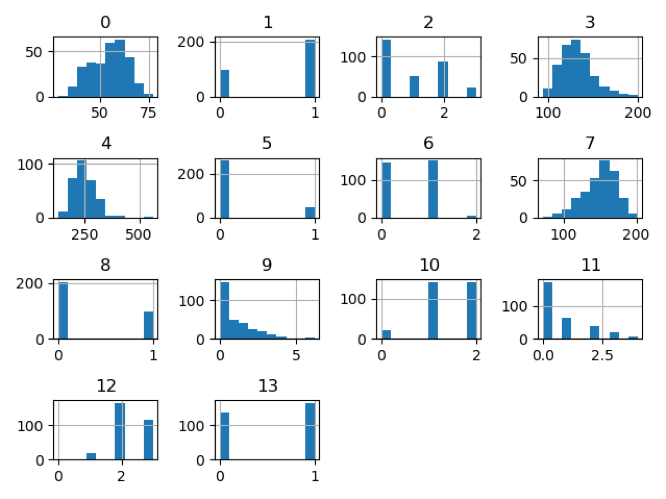
\includegraphics[width=\linewidth]{heart.png}
        \caption{Histograms of Heart Disease. Histogram-0 to Histogram-12 represent the features, Histogram-13 represents the target value.
        X-axis represents the value range and y-axis represents the frequency.}
        \label{histogram of Heart Disease data}
    \end{figure}
    \begin{figure}[h!]
        \includegraphics[width=\linewidth]{imgresults/pulsar_star_hist.png}
        \caption{Histograms of Pulsar Star. Histogram-0 to Histogram-7 represent the features, Histogram-8 represents the target value.
        X-axis represents the value range and Y-axis represents the frequency.}
        \label{histogram of Heart Disease data}
    \end{figure}
    
    
% \subsection{Evaluating using the two data sets}

Among the two data sets, the heart disease data set provides all the potential symptoms of a person with a positive heart disease. 
This database contains 76 attributes, but all distributed tests refer to employing a subset of 14. The objective field alludes to the presence of heart infection within the patient.
The second data set describes a sample of pulsar candidates collected during the High Time Resolution Universe Survey.
Pulsars are a rare type of Neutron star that produce radio emission detectable here on earth. They are of considerable scientific interest as probes of space-time, the inter-stellar medium, and states of matter.
It has gained popularity over recent times to label the pulsar candidates to facilitate rapid analysis. Classification systems in particular are being widely adopted, which treat the candidate data sets as binary classification problems, which is a perfect fit for our comparison.
The histograms of the input data sets have been presented in Fig. 2 and Fig. 3. 
% \figurename  {2} and \figurename {3}. 


We have implemented our VGGMM classifier using cross-validation with the split size of 4 for both the datasets. 
The label for each data point is determined with the largest component among the likelihood of the data point belonging to the classes.
Table 1, presents the model accuracy in comparison with VGMM.



\begin{table}[h!]
    \caption{Model accuracy comparison}
    \begin{center}
    \begin{tabular}{|c|c|c|c|}
    \hline
    \textbf{}&\multicolumn{3}{|c|}{\textbf{Accuracy}} \\
    \cline{2-4} 
    \textbf{\textit{Data set name}}& \textbf{\textit{VGMM}}& \textbf{\textit{VGGMM}} & \textbf{\textit{GMM}}\\
    \hline
    Heart Disease UCI& 41$\%$&69.64$\%$&52$\%$\\
    \hline
    Predicting a Pulsar star& 88$\%$&93.2$\%$&87$\%$\\
    \hline
    % \multicolumn{3}{l}{$^{\mathrm{a}}$Sample of a Table footnote.}
    \end{tabular}
    \label{tab1}
    \end{center}
\end{table}

\subsection{Image Segmentation}
In computer vision, image segmentation is the process of finding the pixels with similar characteristics and clustering them to different segments. The goal of segmentation is to find similar pixels and represent the whole image in the form of segments with each segment representing pixels with similar characteristics making it easier for analysis \cite{b12}\cite{b13}.
\begin{figure}
    \centering
    \begin{subfigure}{.5\linewidth}
      \centering
      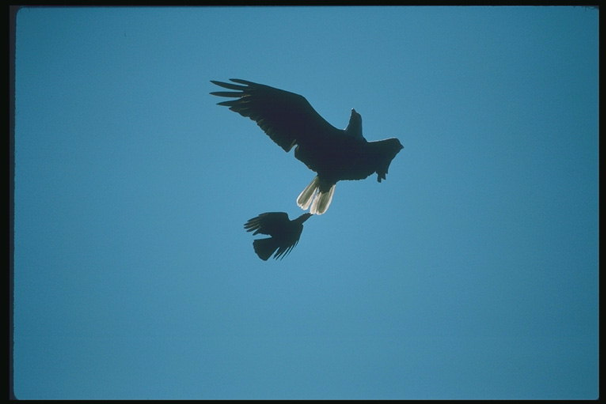
\includegraphics[width=0.9\textwidth]{imgresults/eagle_original.png}
      \caption{Original Image}
      \label{fig:sub1}
    \end{subfigure}%
    \begin{subfigure}{.5\linewidth}
        \centering
        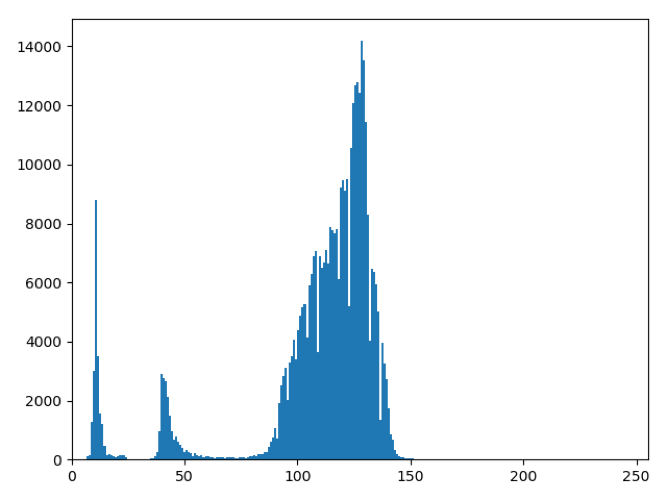
\includegraphics[width=1\textwidth]{imgresults/eagle_hist.png}
        \caption{histogram}
        \label{fig:histogram}
    \end{subfigure}
    \label{fig:sub}


    \begin{subfigure}{.5\linewidth}
        \centering
        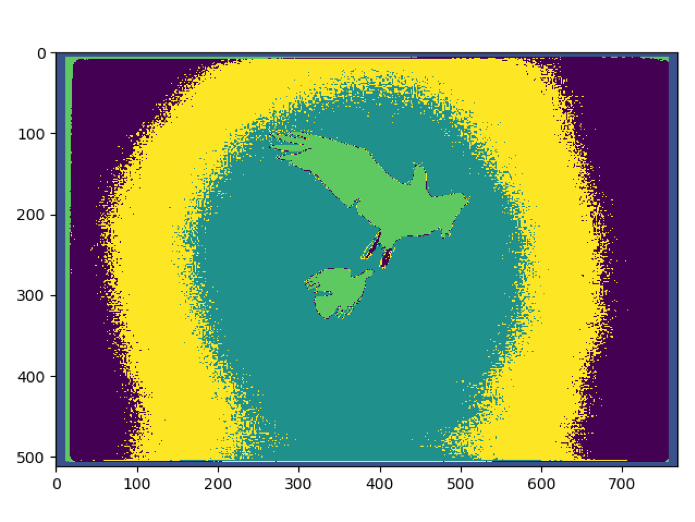
\includegraphics[width=1\textwidth]{imgresults/eagle_kmeans.png}
        \caption{K-means algorithm ($K$=5)}
        \label{fig:sub1}
      \end{subfigure}%
      \begin{subfigure}{.5\linewidth}
          \centering
          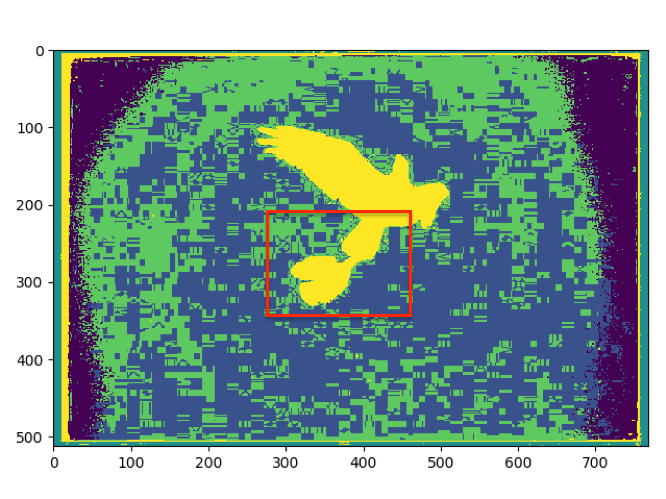
\includegraphics[width=1\textwidth]{imgresults/eagle_gmm.png}
          \caption{GMM ($K$=5)}
          \label{fig:histogram}
      \end{subfigure}
      \label{fig:sub}


    \centering
    \begin{subfigure}{.5\linewidth}
        \centering
        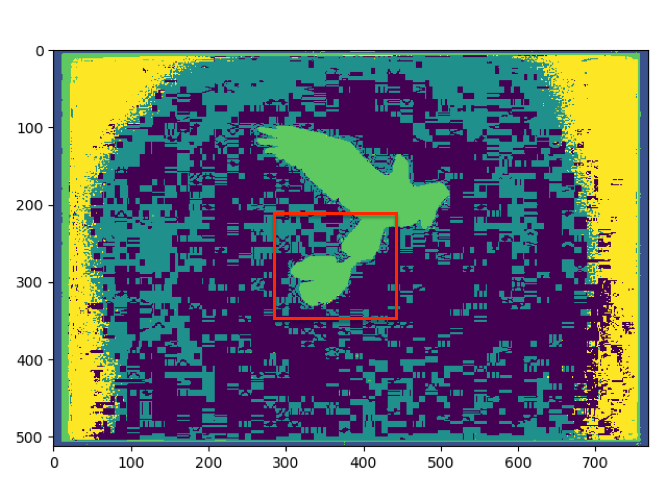
\includegraphics[width=1\textwidth]{imgresults/eagle_vgm.png}
        \caption{VGMM ($K$=5)}
        \label{fig:sub1}
    \end{subfigure}%
    \begin{subfigure}{.5\linewidth}
        \centering
        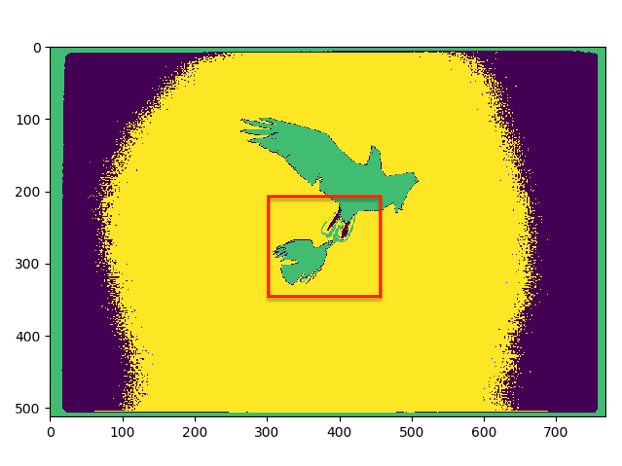
\includegraphics[width=1\textwidth]{imgresults/eagle_vggm.png}
        \caption{VGGMM ($K$=5)}
        \label{fig:sub2}
    \end{subfigure}
    \caption{Segmentation results, Fig. 4a represents the original image.}
    \label{fig:eagle}
\end{figure}


%CROW

\begin{figure}
    \centering
    \begin{subfigure}{.5\linewidth}
      \centering
      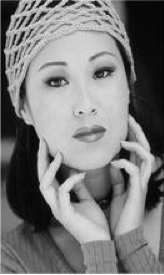
\includegraphics[height=0.7\textwidth]{imgresults/face_original.png}
      \caption{Original Image}
      \label{fig:sub1}
    \end{subfigure}%
    \begin{subfigure}{.5\linewidth}
        \centering
        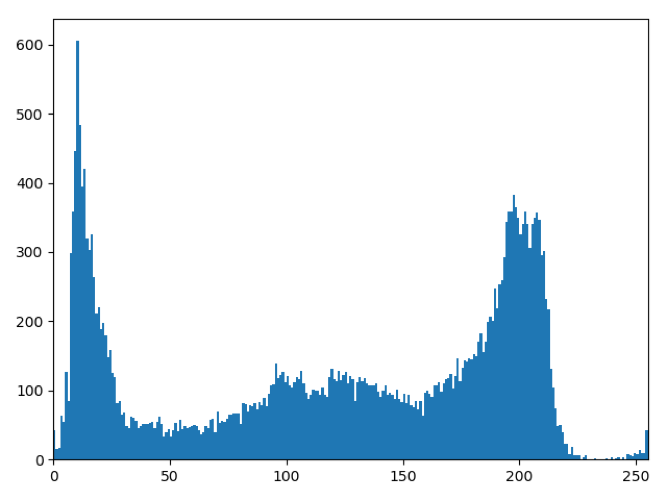
\includegraphics[width=1\textwidth]{imgresults/face_hist.png}
        \caption{histogram}
        \label{fig:histogram}
    \end{subfigure}
    \label{fig:sub}


    \begin{subfigure}{.5\linewidth}
        \centering
        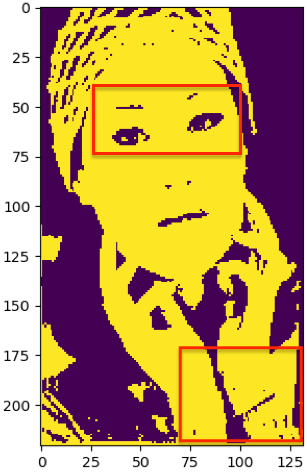
\includegraphics[height=0.7\textwidth]{imgresults/face_kmeans.png}
        \caption{K-means algorithm ($K$=2)}
        \label{fig:sub1}
      \end{subfigure}%
      \begin{subfigure}{.5\linewidth}
          \centering
          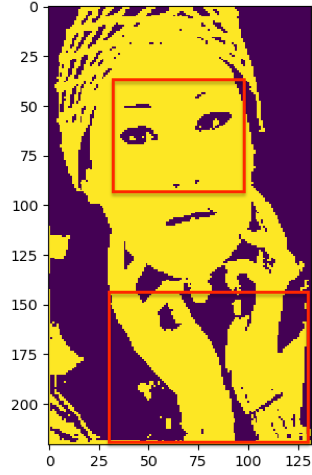
\includegraphics[height=0.7\textwidth]{imgresults/face_gmm.png}
          \caption{GMM ($K$=2)}
          \label{fig:histogram}
      \end{subfigure}
      \label{fig:sub}


    \centering
    \begin{subfigure}{.5\linewidth}
        \centering
        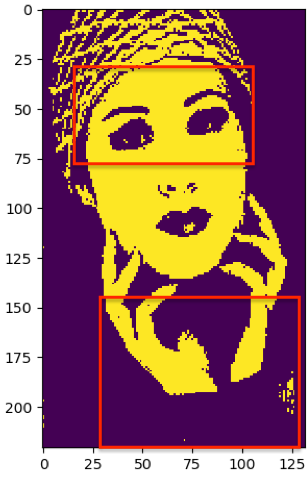
\includegraphics[height=0.7\textwidth]{imgresults/face_vgm.png}
        \caption{VGMM ($K$=2)}
        \label{fig:sub1}
    \end{subfigure}%
    \begin{subfigure}{.5\linewidth}
        \centering
        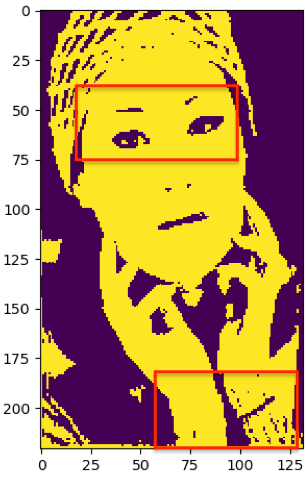
\includegraphics[height=0.7\textwidth]{imgresults/face_vggmm.png}
        \caption{VGGMM ($K$=2)}
        \label{fig:sub2}
    \end{subfigure}
    \caption{Segmentation results, Fig. 5a represents the original image.}
    \label{fig:crow}
\end{figure}
In the first experiment, we choose an image (768 × 512) with two birds in the sky to show the capability to segment small objects in a large background (Fig. 4a). 
The goal is to cluster the image into two classes: the objects with two birds and the sky. 
We set the number of components, $K= 5$.
Comparing the results for K-means algorithm, GMM, and VGMM (Fig. 4c, Fig. 4d, Fig. 4e), there is a large misclassification of the sky and the space between the small object and the large object.
Our method, VGGMM (Fig. 4f), is able to distinguish the two birds and to detect the components effectively. Compared to the other methods, the wings, the tail of the little bird (red square), and the big bird are also shown in more details. 

In the second experiment, we performed our evaluation on a human face image (132 × 221) as shown in Fig. 5a. The goal was to segment the image into two classes. In Fig. 5b, we can see the histogram of the image. 
We set the number of mixture components to two, $K=2$.
Comparing the result with K-means algorithm, GMM, VGMM methods, we noticed that K-means algorithm and GMM have similar results and were able to detect some features of the face. However, they contained only a part of the eyebrows and a part of the texture of clothes rather than the whole. 
VGMM was able to detect the eyebrows but was not able to detect the texture and the hair. 

Our algorithm VGGMM (Fig. 5f), showed more details to offer more information for face recognition and image understanding.

\section{Conclusion}
We have presented a variational inference approach for GGMM. The algorithm is based on treating the shape parameter as a variable. Subsequently, using Binomial Expansion with two cases, we estimate the expectation of the distributions. Hence, the posterior distributions of the inference can be updated by the corresponding hyperparameters.
In the VM-step, the shape parameter is updated using the single-step update of the Newton’s method.


Experimental results show that the VGGMM is an accurate model for medical, astrological, and image segmentation applications by effectively estimating the parameters.
Moreover, in comparison with the VGMM results, the VGGMM has performed better for both classification and image segmentation. 
% in cases of the non gaussian distributed data.
% \subsection{\LaTeX-Specific Advice}
\bibliographystyle{IEEEtran}
\bibliography{ref}
\end{document}
